\documentclass[12pt,a4paper]{article}
\usepackage{amsmath}
\usepackage{amsfonts}
\usepackage{amssymb}
\usepackage{graphicx}
\usepackage{secdot}
\usepackage[left=2cm,right=2cm,top=2cm,bottom=2cm]{geometry}

\author{ Shibayan Biswas, AE21B109\\ Department of Aerospace Engineering\\ IIT Madras}
\title{Homework- 5}
\date{September 27, 2022}
\begin{document}
\maketitle
\hline
\section{Introduction:}
In this particular assignment we have been given certain tasks related to be performed on the integral given below and evaluation of errors is possible as the exact value of the integral is known:
\begin{equation}
	\text{I} = \int_{0}^{\frac{\pi}{2}}{ \text{sin(x)}dx} = 1
\end{equation}
In mathematics, quadrature is a historical term which means the process of determining area. This term is still used nowadays in the context of differential equations, where "solving an equation by quadrature" or "reduction to quadrature" means expressing its solution in terms of integrals. Quadrature problems served as one of the main sources of problems in the development of calculus, and introduce important topics in mathematical analysis.\\
\\The four methods for quadrature as pertinent to this assignment are:
\subsection{Left endpoint method:}
On each sub-interval  [$x_{i-1}$, $xi_$]  (for  i=1,2,3,…,n ), construct a rectangle with width  Δx  and height equal to  f($x_{i-1}$) , which is the function value at the left endpoint of the sub-interval. Then the area of this rectangle is  f($x_{i-1}$)$\Delta$x . The approximation for  integral "I"  is given by adding the area of each rectangle.
\subsection{Right endpoint method:}
Construct a rectangle on each sub-interval  [$x_{i-1}$, $x_i$] , only this time the height of the rectangle is determined by the function value  f($x_i$)  at the right endpoint of the sub-interval. Then, the area of each rectangle is  f($x_i$)$\Delta$x  and the approximation for  integral "I"  is given by adding the area of each rectangle.
\subsection{Mid point theorem:}
A third way to estimate the area under a graph is to set the height of each rectangle equal to the value of f at the midpoint of each sub-interval, obtaining the midpoint estimate. Specifically, above the interval [$x_$0, $x_1$] there is again a rectangle of width $\Delta$x, but its height is the value of $f$ at the midpoint of the interval. The midpoint is $\frac{\text{($x_0$+$x_1$)}}{\text{2}}$, so the height is f($\frac{\text{($x_0$+$x_1$)}}{\text{2}}$) and the area of the rectangle is f($\frac{\text{($x_0$+$x_1$)}}{\text{2}}$)$\Delta$x. Similarly, above each interval [$x_{j-1}$,$x_j$], which has midpoint $\frac{\text{($x_{j-1}$+$x_j$)}}{\text{2}}$, there is a rectangle of width $\Delta$x and height f($\frac{\text{($x_{j-1}$+$x_j$)}}{\text{2}}$), and hence of area f($\frac{\text{($x_{j-1}$+$x_j$)}}{\text{2}}$)$\Delta$x. The approximation for  integral "I"  is given by adding the area of each rectangle.
\subsection{Trapezoidal Method:}
We need not restrict ourselves to rectangles. Instead, we could plot the points on the graph y=f(x) for each $x_j$, and join the dots. In this way, the function f(x) is approximated by a piece-wise linear function, that is, a sequence of straight line segments. The area under y=f(x) is then approximated by trapezia. This estimate is known as the trapezoidal estimate.\\
\\Above the interval [$x_0$, $x_1$] we have a trapezium of width $\frac{b-a}{n} = \Delta x$. Its left side has height f($x_0$), and its right side has height f($x_1$). So the area of the trapezium is ($\frac{\text{\text{f}($x_0$)+\text{f}($x_1$)}}{\text{2}}$). Similarly, above the interval [$x_{j-1}$, $x_j$], we have a trapezium of width $\Delta$x with two sides of height f($x_{j-1}$) and f($x_j$), hence the area of the trapezium is ($\frac{\text{\text{f}($x_{j-1}$)+\text{f}($x_j$)}}{\text{2}}$)$\Delta$x. The approximation for  integral "I"  is given by adding the area of each trapezium.
\section{Plot of Absolute Error v/s $\Delta$x:}
In the following section I have represented the plot of Absolute Error v/s $\Delta$x while approximating the value of the integral "I" by using the Left endpoint, Right endpoint, Mid point and Trapezoidal Method. The plot is shown below:
\begin{figure}[!ht]
	\begin{center}
		\framebox{
			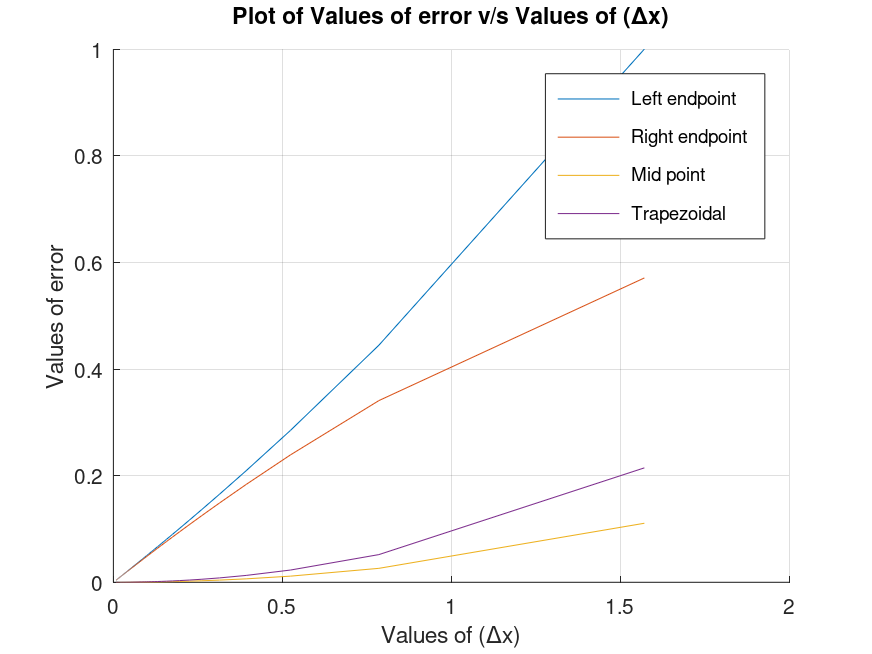
\includegraphics[scale=0.5]{Figure_1.png}
		}
	\end{center}
	\caption{Plot of Absolute Error v/s $\Delta$x}
\end{figure}
\section{Plot of Logarithm of Error v/s Logarithm of $\Delta$x:}
In the following section I have represented the plot of Logarithm of Error v/s Logarithm of $\Delta$x while approximating the value of the integral "I" by using the Left endpoint, Right endpoint, Mid point and Trapezoidal Method. The plot is shown below:
\begin{figure}[!ht]
	\begin{center}
		\framebox{
			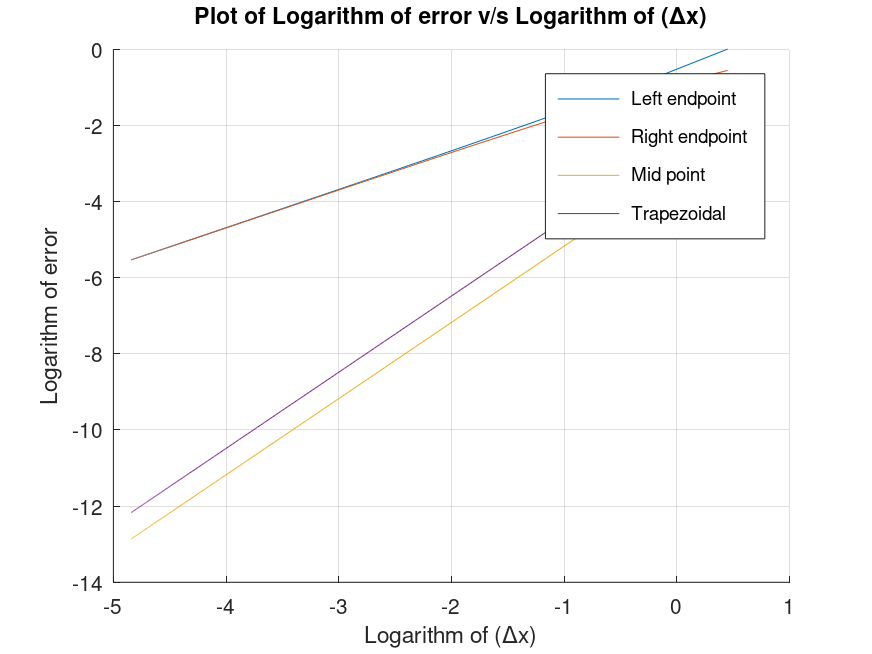
\includegraphics[scale=0.5]{Figure_2.png}
		}
	\end{center}
	\caption{Plot of Logarithm of Error v/s Logarithm of $\Delta$x}
\end{figure}
\section{Plot of Best fit Lines using Linear Regression:}
In the following section I have represented the plot of the Best fit Lines using Linear Regression for the plot of Absolute Error v/s $\Delta$x while approximating the value of the integral "I" by using the Left endpoint, Right endpoint, Mid point and Trapezoidal Method. The plot is shown below:
\clearpage
\begin{figure}[h]
	\begin{center}
		\framebox{
			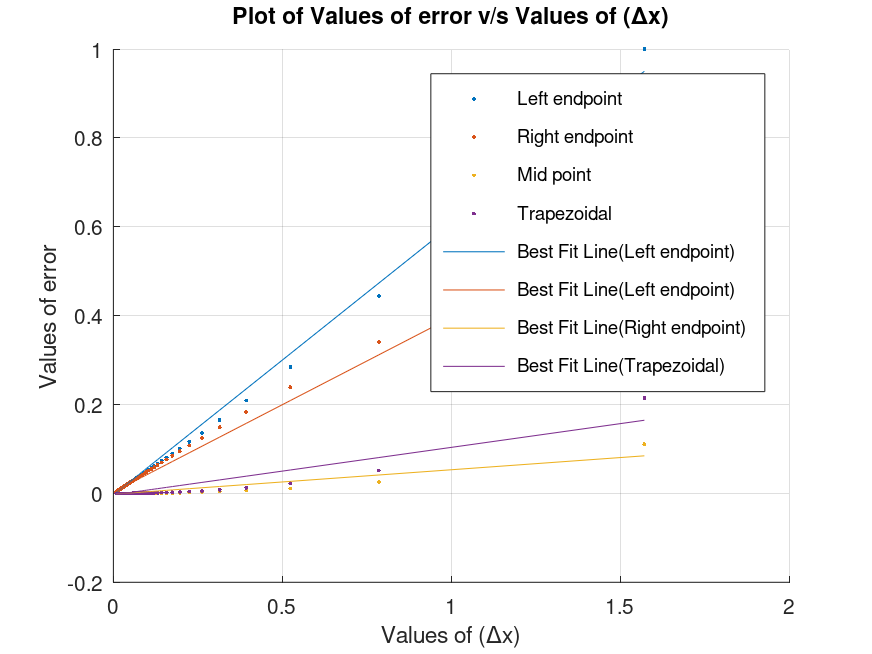
\includegraphics[scale=0.5]{Figure_3.png}
		}
	\end{center}
	\caption{Plot of Best fit Lines using Linear Regression}
\end{figure}
\noindent
Linear Regression is a statistical method used in finance, investing, and other disciplines that attempts to determine the strength and character of the relationship between one dependent variable (usually denoted by Y) and a series of other variables (known as independent variables).\\
\\Also called simple regression or ordinary least squares, linear regression is the most common form of this technique. Linear regression establishes the linear relationship between two variables based on a line of best fit. Linear regression is thus graphically depicted using a straight line with the slope defining how the change in one variable impacts a change in the other. The y-intercept of a linear regression relationship represents the value of one variable when the value of the other is zero. 
\section{Inferences from the Linear Regression Model:}
In this section I have written some facts from the analysis of the above plot of the Best fit Lines using Linear Regression for the plot of Absolute Error v/s $\Delta$x while approximating the value of the integral "I" by using the Left endpoint, Right endpoint, Mid point and Trapezoidal Method.\\
\\In the above plot I have tried to plot the Best Fit Lines for the scatter plots of Absolute Error v/s $\Delta$x by using Linear Regression. As we can see, for none of the cases, the linear regression resulted in a straight line. The slope of the Best Fit Lines obtained by linear regression indicates the Values of error for a given interval $\Delta$x. I would want a scheme with lower value of slope in order to get a lesser Value of error for a given interval $\Delta$x.
\section{Plot $I_{LE}$ and $I_{RE}$ as function of $\Delta$x:}
In the following section I have represented the plot $I_{LE}$ and $I_{RE}$ as function of $\Delta$x while approximating the value of the integral "I" by using the Left endpoint and Right endpoint method. The plot is shown below:
\begin{figure}[h]
	\begin{center}
		\framebox{
			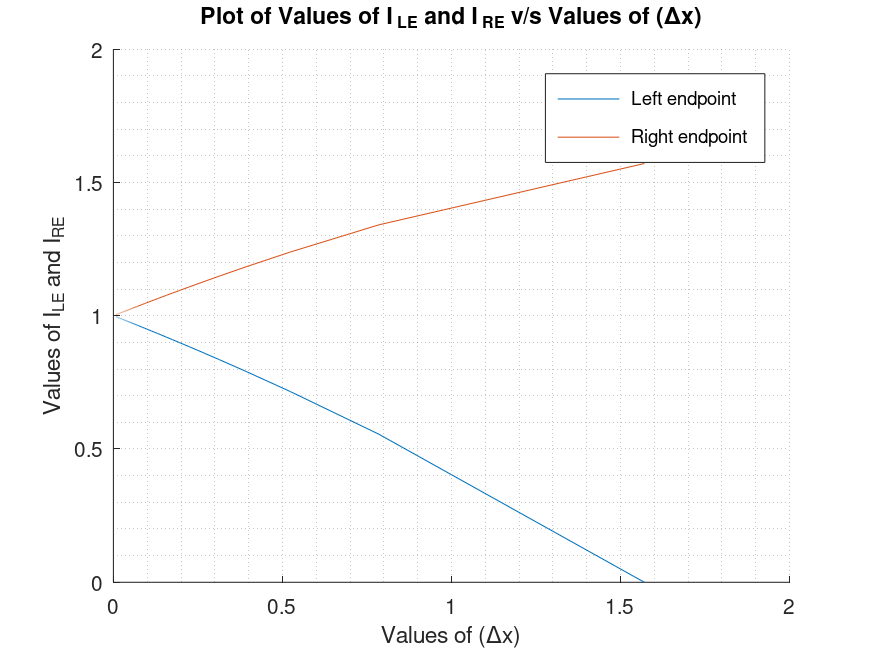
\includegraphics[scale=0.55]{Figure_4.png}
		}
	\end{center}
	\caption{Plot $I_{LE}$ and $I_{RE}$ as function of $\Delta$x}
\end{figure}
\\As the number of segments tend to infinity, the value of the integral "I" tends to the correct value that is obtained mathematically and for this case $	\text{I} = \int_{0}^{\frac{\pi}{2}}{ \text{sin(x)}dx} = 1$. In this particular case the Value of error = 0.
\section{Plot of Computational Cost for each method:}
In the following section I have represented the plot of Computational Cost for each method while approximating the value of the integral "I" by using the Left endpoint, Right endpoint, Mid point and Trapezoidal Method. The plot is shown below:
\clearpage
\begin{figure}[!ht]
	\begin{center}
		\framebox{
			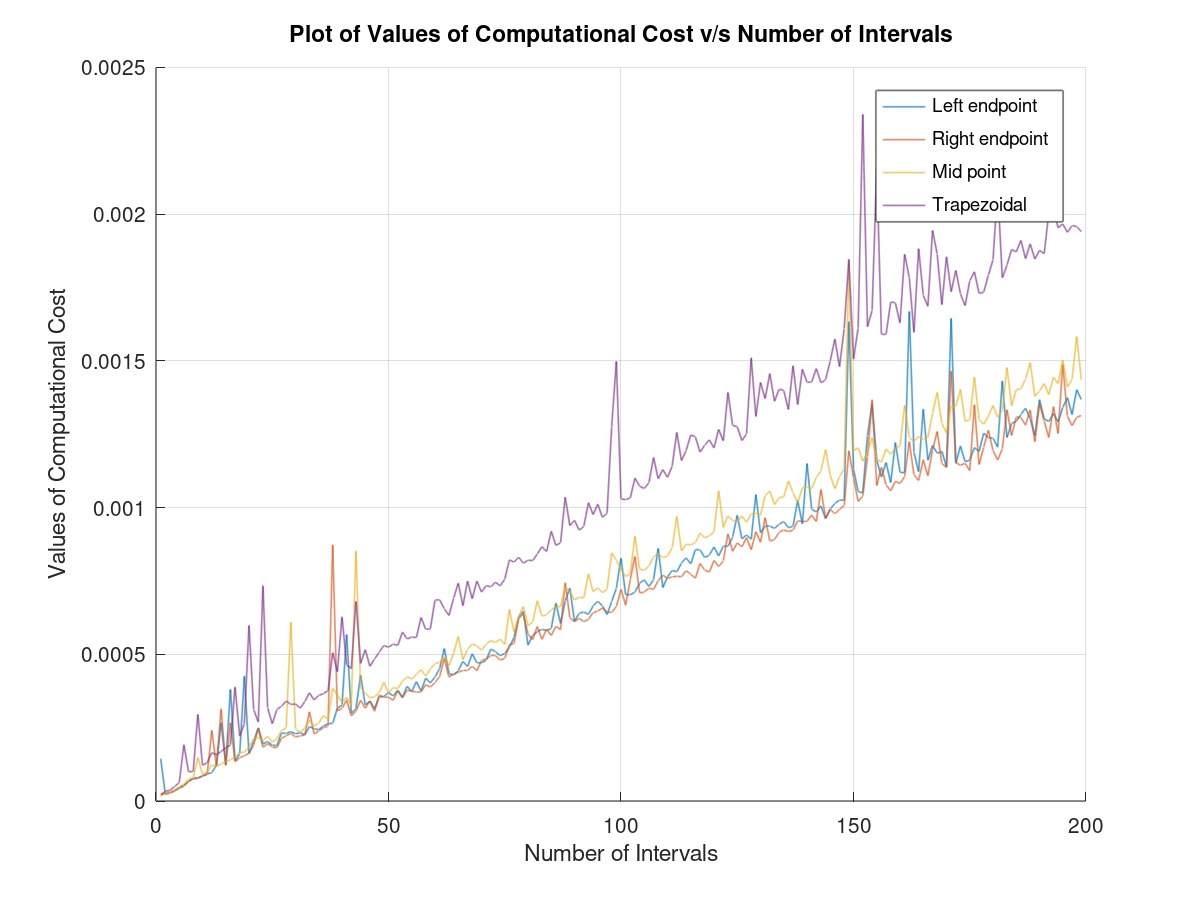
\includegraphics[scale=0.4]{Figure_5.png}
		}
	\end{center}
	\caption{Plot of Computational Cost for each method}
\end{figure}
\noindent
From the above plot I infer that the Computational Cost is the least for the Right endpoint method, followed by the Left endpoint method, followed by the Midpoint method and followed by the Trapezoidal method. From the above plot we notice that the Right endpoint method has the least Computational Cost among all the methods and the Trapezoidal method has the most Computational Cost among all the methods.
\end{document}
